\documentclass[12pt,letterpaper,final]{article}

%\documentstyle[12pt,graphicx,natbib,hyperref,Sweave,rotating]{article}

\usepackage{Sweave}
\usepackage{graphicx}
\usepackage{natbib}
\usepackage{hyperref}
\usepackage{caption}
\usepackage{rotating}
\usepackage{verbatim}
\usepackage{textcomp}

\setlength{\oddsidemargin}{0in}
\setlength{\textwidth}{6.15in}
\setlength{\topmargin}{0.5in}
\setlength{\textheight}{22cm}
\setlength{\headheight}{0in}
\setlength{\headsep}{0in}
\setlength{\parskip}{5pt plus 2pt minus 3pt}

\marginparwidth2cm
\marginparsep0.2cm
\marginparpush0.2cm
%\tabcolsep0pt

\def\thefootnote{\fnsymbol{footnote}}
\setcounter{footnote}{1}

\renewcommand{\baselinestretch}{1.2}
\renewcommand{\labelenumi}{(\roman{enumi})}

\renewcommand{\topfraction}{1.0}
\renewcommand{\bottomfraction}{1.0}
\renewcommand{\textfraction}{0.0}
\renewcommand{\floatpagefraction}{1.0}

\newtheorem{definition}{Definition}
\newtheorem{theorem}{Theorem}
\newtheorem{lemma}[theorem]{Lemma}
\newtheorem{claim}[theorem]{Claim}
\newtheorem{fact}[theorem]{Fact}

% to get nice proofs ...
\newcommand{\qedsymb}{\mbox{ }~\hfill~{\rule{2mm}{2mm}}}
\newenvironment{proof}{\begin{trivlist}
\item[\hspace{\labelsep}{\bf\noindent Proof: }]
}{\qedsymb\end{trivlist}}

\def\printindex{\input{\jobname.ind}}

\newfont{\msymb}{cmsy10 scaled 1000}

\def\nullset{\mbox{\O}}
\def\R{{I\!\!R}}
\def\N{{I\!\!N}}
\def\C{{C\!\!\!\!I}}

\def\convdist{\stackrel{d}{\longrightarrow}}
\def\convlaw{\stackrel{L}{\longrightarrow}}
\def\convweak{\stackrel{w}{\longrightarrow}}
\def\convprob{\stackrel{p}{\longrightarrow}}
\def\convmean#1{\stackrel{#1}{\longrightarrow}}
\def\convas{\stackrel{a.s.}{\longrightarrow}}
\def\convwp{\stackrel{w.p.1}{\longrightarrow}}

\def\A{\mbox{\msymb A}}
\def\B{\mbox{\msymb B}}
\def\H{\mbox{\msymb H}}
\def\P{\mbox{\msymb P}}
\def\S{\mbox{\msymb S}}
\def\X{\mbox{\msymb X}}
\def\Y{\mbox{\msymb Y}}

\def\u0{\underline{0}}
\def\ua{\underline{a}}
\def\ub{\underline{b}}
\def\ud{\underline{d}}
\def\ug{\underline{g}}
\def\ueta{\underline{\eta}}
\def\umu{\underline{\mu}}
\def\utheta{\underline{\theta}}
\def\uvartheta{\underline{\vartheta}}
\def\UT{\underline{T}}
\def\ut{\underline{t}}
\def\UU{\underline{U}}
\def\uu{\underline{u}}
\def\OX{\overline{X}}
\def\UX{\underline{X}}
\def\ux{\underline{x}}
\def\UY{\underline{Y}}
\def\uy{\underline{y}}
\def\UZ{\underline{Z}}
\def\uz{\underline{z}}

%\parskip 0.1in
\pagenumbering{arabic}    %  Start using 1,2,... as page numbers.
\pagestyle{plain}         %  Page numbers in middle bottom of page.
%\setcounter{page}{80}  % XXXXXXXXXXXXXXXXX
%\setcounter{theorem}{5} % XXXXXXXXXXXXXXXXX
%\setcounter{definition}{10} % XXXXXXXXXXXXXXXXX

\parindent 0in

\makeindex


\begin{document}

\Sconcordance{concordance:lect_main.tex:lect_main.Rnw:%
1 164 1}
\Sconcordance{concordance:lect_main.tex:./lect_acknow.Rnw:ofs 165:%
1 40 1}
\Sconcordance{concordance:lect_main.tex:lect_main.Rnw:ofs 206:%
167 13 1}
\Sconcordance{concordance:lect_main.tex:./lect_chapter6.Rnw:ofs 220:%
1 27 1 1 2 12 0 3 1 2 2 1 3 1 0 1 3 1 0 1 1 1 3 1 0 1 1 1 3 1 0 1 1 4 0 %
1 2 6 1 1 2 1 0 1 1 1 3 1 0 1 4 2 0 1 4 2 0 1 5 3 0 1 2 4 0 1 2 15 1 1 %
2 1 0 2 2 1 1 1 2 1 0 1 2 1 1 1 2 1 0 1 2 1 1 1 2 1 0 1 2 1 1 1 2 1 0 1 %
2 1 1 1 2 1 0 1 2 1 1 1 2 5 0 1 2 10 1 1 2 1 0 1 3 1 0 1 1 1 2 1 3 1 0 %
1 1 1 3 1 0 1 1 1 3 1 0 1 1 4 0 1 2 1 1 1 2 1 0 1 1 1 2 1 8 6 0 1 8 6 0 %
1 1 3 0 1 2 1 1 1 9 8 0 1 1 3 0 1 2 1 1 1 7 6 0 1 1 3 0 1 2 1 1 1 2 5 0 %
1 2 21 1 1 2 1 0 1 1 1 2 4 0 2 2 5 0 2 2 5 0 2 2 5 0 2 2 5 0 2 2 5 0 1 %
2 3 1 1 2 1 0 1 1 1 5 3 0 1 1 3 0 1 2 1 1 1 5 4 0 1 1 3 0 1 2 1 1 1 2 5 %
0 1 2 11 1 1 47 49 0 1 2 8 1 1 2 1 0 1 1 1 2 5 0 1 2 5 0 1 2 6 0 1 2 5 %
1 4 0 1 3 5 1 1 2 6 0 1 2 1 4 6 0 1 2 29 1}
\Sconcordance{concordance:lect_main.tex:lect_main.Rnw:ofs 698:%
182 28 1}



\bibliographystyle{agsm}

\begin{titlepage}
\vspace*{4.5cm}
\begin{center}
{\LARGE \bf Stat 5810, Section 003} \\[0.5cm]
{\LARGE \bf Statistical Visualization I} \\[0.5cm]
{\LARGE \bf Fall 2018} \\[0.5cm]
~ \\[2cm]
{\bf Dr. J\"urgen Symanzik} \\[0.3cm]
Utah State University \\[0.3cm]
Department of Mathematics and Statistics \\[0.3cm]
3900 Old Main Hill \\[0.3cm]
Logan, UT 84322--3900 \\[0.8cm]
Tel.: (435) 797--0696 \\[0.3cm]
FAX: (435) 797--1822 \\[0.3cm]
e-mail: \verb|symanzik@math.usu.edu| \\[0.3cm]
Web: \url{http://www.math.usu.edu/~symanzik/}
\end{center}

\thispagestyle{empty}
\vfill
\end{titlepage}

\newpage

\thispagestyle{empty}

\vspace*{5cm}

\begin{figure}[ht]
\centering{\includegraphics[width=0.99\textwidth]{Scans//PhdcomicsCom_Plotting.jpg}}
\caption{\label{PhdcomicsCom_Plotting}
\url{http://www.phdcomics.com/comics/archive.php?comicid=1541}, \\
Cartoon.
}
\end{figure}


\newpage


\setcounter{page}{1}

\tableofcontents

\newpage

%~
%
%\newpage

% !Rnw root = lect_main.Rnw

\section*{Acknowledgements}

This course uses some of the course materials provided by
Dr.\ Mike Minnotte (formerly USU, now with the University of
North Dakota) as held in the Fall 2006 semester. Additional materials
have been taken from other Statistical Graphics courses, such as the
ones offered by Dr.\ Di Cook (formerly Iowa State University; now Monash University:
\url{http://dicook.org/}) and
Dr.\ Dan Carr (George Mason University: \url{http://mason.gmu.edu/~dcarr/}).
Other examples and R code originate from 
Heike Hofmann, Paul Murrell, Carson Sievert,
Martin Theus, Antony Unwin, Simon Urbanek, 
Hadley Wickham, Lee Wilkinson, and others.
We are likely to include parts from additional authors and sources
that will be specified later during the semester.

Thanks are also due to 60+ students and guests who took 
the former ``Stat 6560: Graphical Methods'' and
the current ``Statistical Visualization I \& II'' courses
with me since the Spring 2009 semester 
for their valuable comments that helped
to improve, correct, and extend these lecture notes.

~\\
J\"urgen Symanzik, September 10, 2018.


\begin{figure}[ht]
\centering{\includegraphics[width=3.5in]{Scans//Zelazny_px_Fig.jpg}}
\caption{\label{Zelazny_px_Fig}
\cite{Ze2001}, p.~x, Cartoon.
}
\end{figure}

\newpage

%~\\
%
%\newpage
\addcontentsline{toc}{section}{Acknowledgements}

\newpage


\setcounter{page}{1}

% !Rnw root = lect_main.Rnw

\def\jsprivatechzero{1} % show additional details
%\def\jsprivatechzero{0} % do NOT show additional details



\section{Introduction}


\subsection{Goals of the Course}

The course answers three main questions: 
\begin{itemize}
\item Q: Why statistical graphics (and which ones to draw)? --- \\
A: \cite{Un2015}, p.~xi, indicates that statistical graphics can be used for
\begin{itemize}
\item data cleaning
\item exploring the data structure
\item detecting outliers and unusual groups
\item identifying trends and clusters
\item spotting local patterns
\item evaluating modeling output
\item presenting results
\item exploratory data analysis (EDA)
\item data mining
\end{itemize}

Different types of graphics answer different questions. Often, we draw a large
number of (different) graphics to better understand the full data set.


\item Q: How to construct statistical graphics in R? --- \\
A: Many R packages and supporting books exists, e.g.,
\begin{itemize}
\item baseR, see \cite{RCore2017}
\item {\tt ggplot2}, see \cite{WiCh2016} and \cite{Wick2009}
\item {\tt lattice}, see \cite{Sar2017} and \cite{Sar2008}
\item general overview of R graphics, see \cite{Mu2006}
\end{itemize}
This course is not about a single R package, but rather introduces, uses, and compares
a large number of R packages for various types of graphics.

\item Q: How to distinguish between {\bf good} and {\bf bad} statistical graphics? --- \\
A: see the next section for a first brief answer 
\end{itemize}


\subsection{Motivation: Bad Graphics}

Statistical graphics and data visualization are critical 
elements of modern data analysis and presentation.  From initial
exploration of a data set to the final presentation of results to
the end user, statistical graphics play a vital role in shaping our understanding
of our data.  Through proper use of graphics, we can make critical
discoveries, and communicate them clearly.  Conversely, poor use
or misuse of graphics can seriously mislead (by accident or design).

In the recent past, three examples that show the misuse of statistical graphics
have been widely discussed --- in the statistical community and beyond.


\newpage


\underline{Example 1:}


\begin{figure}[ht]
\centering{\includegraphics[width=3.5in]{Scans//FoxNews_Bush-cuts2013.png}}
\caption{\label{FoxNews_Bush-cuts2013}
Figure taken from
\url{http://flowingdata.com/2012/08/06/fox-news-continues-charting-excellence/}
on 9/13/2017.
}
\end{figure}


Based on this graphic (and without looking at the axis labels and percentages)
how much higher would the top tax rate be if the Bush tax cuts were to expire
at the end of 2012? Really ?!?!?


\begin{figure}[ht]
\centering{\includegraphics[width=2.0in]{Scans//FoxNews_Bush-cuts2013_corrected.png}}
\caption{\label{FoxNews_Bush-cuts2013_corrected}
Corrected figure taken from
\url{http://flowingdata.com/2012/08/06/fox-news-continues-charting-excellence/}
on 9/13/2017.
}
\end{figure}


\newpage


\underline{Example 2:}


\begin{figure}[ht]
\centering{\includegraphics[width=3.5in]{Scans//Obamacare1.pdf}}
\caption{\label{Obamacare1}
Figure taken from
\url{https://www.mediamatters.org/blog/2014/03/31/dishonest-fox-charts-obamacare-enrollment-editi/198679}
on 3/31/2014.
}
\end{figure}


Based on this graphic (and without looking at the numbers in the graphic)
how much of the target Obamacare enrollment has been reached 4 days prior to the 
March 31 deadline? Really ?!?!?


\begin{figure}[ht]
\centering{\includegraphics[width=4.5in]{Scans//Obamacare2.jpg}}
\caption{\label{Obamacare2}
Corrected figure taken from \cite{HRS2014}, Figure~10, showing the ``tip of
the iceberg'' of the bar chart.
}
\end{figure}


\newpage


\underline{Example 3:}


\begin{figure}[ht]
\centering{\includegraphics[width=3.8in]{Scans//PlannedParenthood1.jpg}}
\caption{\label{PlannedParenthood1}
Rep.\ Jason Chaffetz, R-Utah, projected this chart during a high-profile congressional hearing investigating Planned Parenthood.
Figure taken from
\url{http://www.politifact.com/truth-o-meter/statements/2015/oct/01/jason-chaffetz/chart-shown-planned-parenthood-hearing-misleading-/}
on 10/12/2017.
}
\end{figure}

What is Planned Parenthood mostly doing in 2013, according to Rep.\ Jason Chaffetz, R-Utah?
Really ?!?!?

\begin{figure}[ht]
\centering{\includegraphics[width=5.5in]{Scans//PlannedParenthood2.jpg}}
\caption{\label{PlannedParenthood1}
Figure taken from
\url{http://www.politifact.com/truth-o-meter/statements/2015/oct/01/jason-chaffetz/chart-shown-planned-parenthood-hearing-misleading-/}
on 10/12/2017. 
}
\end{figure}


\newpage


\begin{figure}[ht]
\centering{\includegraphics[width=5.0in]{Scans//PlannedParenthood3.png}}
\caption{\label{PlannedParenthood1}
Corrected figure taken from
\url{http://www.politifact.com/truth-o-meter/statements/2015/oct/01/jason-chaffetz/chart-shown-planned-parenthood-hearing-misleading-/}
on 10/12/2017. 
}
\end{figure}


Politifact concluded: 
\begin{quotation}
``At the hearing, Chaffetz presented a chart that showed the number of abortions at Planned Parenthood rising higher than the number of preventive services and cancer screenings between 2006 and 2013.

But that's inaccurate, disputed by the chart's own, hard to read numerical labels. In fact, there were three times as many cancer screenings and prevention services as abortions in 2013. Experts in data presentation said this was an egregious example of using a chart to mislead.

We rate the claim Pants on Fire.''
\end{quotation}


\newpage


\subsection{Motivation: Why Graphics ?!?}

Why do we need graphics at all. Aren't summary statistics sufficient? 

Start R and load the \citet{Ans73} data sets. Just type \verb|anscombe|
and take a first glance at the data sets. What do you notice?
\begin{Schunk}
\begin{Sinput}
> anscombe
\end{Sinput}
\begin{Soutput}
   x1 x2 x3 x4    y1   y2    y3    y4
1  10 10 10  8  8.04 9.14  7.46  6.58
2   8  8  8  8  6.95 8.14  6.77  5.76
3  13 13 13  8  7.58 8.74 12.74  7.71
4   9  9  9  8  8.81 8.77  7.11  8.84
5  11 11 11  8  8.33 9.26  7.81  8.47
6  14 14 14  8  9.96 8.10  8.84  7.04
7   6  6  6  8  7.24 6.13  6.08  5.25
8   4  4  4 19  4.26 3.10  5.39 12.50
9  12 12 12  8 10.84 9.13  8.15  5.56
10  7  7  7  8  4.82 7.26  6.42  7.91
11  5  5  5  8  5.68 4.74  5.73  6.89
\end{Soutput}
\end{Schunk}

Then calculate some summary statistics (separately for the 
four columns of X's and Y's):
mean of the X's, mean of the Y's, 
standard deviation of the X's, standard deviation of the Y's,
correlation coefficient,
slope and intercept of the regression line, rms error.

%\url{http://www.math.usu.edu/~symanzik/teaching/2015_stat6560/RDataAndScripts/Anscombe.R}

\begin{Schunk}
\begin{Sinput}
> # calculate some summary statistics (separately for the 
> # four columns of X's and Y's)
> 
> # mean of the X's
> mean(anscombe$x1)
\end{Sinput}
\begin{Soutput}
[1] 9
\end{Soutput}
\begin{Sinput}
> mean(anscombe$x2)
\end{Sinput}
\begin{Soutput}
[1] 9
\end{Soutput}
\begin{Sinput}
> mean(anscombe$x3)
\end{Sinput}
\begin{Soutput}
[1] 9
\end{Soutput}
\begin{Sinput}
> mean(anscombe$x4)
\end{Sinput}
\begin{Soutput}
[1] 9
\end{Soutput}
\begin{Sinput}
> # mean of the Y's
> mean(anscombe$y1)
\end{Sinput}
\begin{Soutput}
[1] 7.500909
\end{Soutput}
\begin{Sinput}
> mean(anscombe$y2)
\end{Sinput}
\begin{Soutput}
[1] 7.500909
\end{Soutput}
\begin{Sinput}
> mean(anscombe$y3)
\end{Sinput}
\begin{Soutput}
[1] 7.5
\end{Soutput}
\begin{Sinput}
> mean(anscombe$y4)
\end{Sinput}
\begin{Soutput}
[1] 7.500909
\end{Soutput}
\begin{Sinput}
> # standard deviation of the X's
> sqrt(var(anscombe$x1))
\end{Sinput}
\begin{Soutput}
[1] 3.316625
\end{Soutput}
\begin{Sinput}
> sqrt(var(anscombe$x2))
\end{Sinput}
\begin{Soutput}
[1] 3.316625
\end{Soutput}
\begin{Sinput}
> sqrt(var(anscombe$x3))
\end{Sinput}
\begin{Soutput}
[1] 3.316625
\end{Soutput}
\begin{Sinput}
> sqrt(var(anscombe$x4))
\end{Sinput}
\begin{Soutput}
[1] 3.316625
\end{Soutput}
\begin{Sinput}
> # standard deviation of the Y's
> sqrt(var(anscombe$y1))
\end{Sinput}
\begin{Soutput}
[1] 2.031568
\end{Soutput}
\begin{Sinput}
> sqrt(var(anscombe$y2))
\end{Sinput}
\begin{Soutput}
[1] 2.031657
\end{Soutput}
\begin{Sinput}
> sqrt(var(anscombe$y3))
\end{Sinput}
\begin{Soutput}
[1] 2.030424
\end{Soutput}
\begin{Sinput}
> sqrt(var(anscombe$y4))
\end{Sinput}
\begin{Soutput}
[1] 2.030579
\end{Soutput}
\begin{Sinput}
> # correlation coefficient
> cor(anscombe$x1, anscombe$y1)
\end{Sinput}
\begin{Soutput}
[1] 0.8164205
\end{Soutput}
\begin{Sinput}
> cor(anscombe$x2, anscombe$y2)
\end{Sinput}
\begin{Soutput}
[1] 0.8162365
\end{Soutput}
\begin{Sinput}
> cor(anscombe$x3, anscombe$y3)
\end{Sinput}
\begin{Soutput}
[1] 0.8162867
\end{Soutput}
\begin{Sinput}
> cor(anscombe$x4, anscombe$y4)
\end{Sinput}
\begin{Soutput}
[1] 0.8165214
\end{Soutput}
\begin{Sinput}
> # slope of the regression line
> slope1 <- cor(anscombe$x1, anscombe$y1) * sqrt(var(anscombe$y1)) / 
+   sqrt(var(anscombe$x1))
> slope2 <- cor(anscombe$x2, anscombe$y2) * sqrt(var(anscombe$y2)) / 
+   sqrt(var(anscombe$x2))
> slope3 <- cor(anscombe$x3, anscombe$y3) * sqrt(var(anscombe$y3)) / 
+   sqrt(var(anscombe$x3))
> slope4 <- cor(anscombe$x4, anscombe$y4) * sqrt(var(anscombe$y4)) / 
+   sqrt(var(anscombe$x4))
> slope1
\end{Sinput}
\begin{Soutput}
[1] 0.5000909
\end{Soutput}
\begin{Sinput}
> slope2
\end{Sinput}
\begin{Soutput}
[1] 0.5
\end{Soutput}
\begin{Sinput}
> slope3
\end{Sinput}
\begin{Soutput}
[1] 0.4997273
\end{Soutput}
\begin{Sinput}
> slope4
\end{Sinput}
\begin{Soutput}
[1] 0.4999091
\end{Soutput}
\begin{Sinput}
> # intercept of the regression line
> intercept1 <- mean(anscombe$y1) - slope1 * mean(anscombe$x1)
> intercept2 <- mean(anscombe$y2) - slope2 * mean(anscombe$x2)
> intercept3 <- mean(anscombe$y3) - slope3 * mean(anscombe$x3)
> intercept4 <- mean(anscombe$y4) - slope4 * mean(anscombe$x4)
> intercept1
\end{Sinput}
\begin{Soutput}
[1] 3.000091
\end{Soutput}
\begin{Sinput}
> intercept2
\end{Sinput}
\begin{Soutput}
[1] 3.000909
\end{Soutput}
\begin{Sinput}
> intercept3
\end{Sinput}
\begin{Soutput}
[1] 3.002455
\end{Soutput}
\begin{Sinput}
> intercept4
\end{Sinput}
\begin{Soutput}
[1] 3.001727
\end{Soutput}
\begin{Sinput}
> # rms error
> rmserror1 <- sqrt(1 - cor(anscombe$x1, anscombe$y1)^2) * sqrt(var(anscombe$y1))
> rmserror2 <- sqrt(1 - cor(anscombe$x2, anscombe$y2)^2) * sqrt(var(anscombe$y2))
> rmserror3 <- sqrt(1 - cor(anscombe$x3, anscombe$y3)^2) * sqrt(var(anscombe$y3))
> rmserror4 <- sqrt(1 - cor(anscombe$x4, anscombe$y4)^2) * sqrt(var(anscombe$y4))
> rmserror1
\end{Sinput}
\begin{Soutput}
[1] 1.173145
\end{Soutput}
\begin{Sinput}
> rmserror2
\end{Sinput}
\begin{Soutput}
[1] 1.173724
\end{Soutput}
\begin{Sinput}
> rmserror3
\end{Sinput}
\begin{Soutput}
[1] 1.172868
\end{Soutput}
\begin{Sinput}
> rmserror4
\end{Sinput}
\begin{Soutput}
[1] 1.172284
\end{Soutput}
\end{Schunk}


So, the four pairs of X/Y columns basically are identical !?!


\if\jsprivatechzero 1
But, didn't we forget to {\bf plot} the data !!! 

%\url{http://www.math.usu.edu/~symanzik/teaching/2015_stat6560/RDataAndScripts/Anscombe2.R}

\begin{Schunk}
\begin{Sinput}
> # based on: http://pbil.univ-lyon1.fr/library/base/html/anscombe.html
> # extracted and adapted on 1/6/09
> 
> ##-- now some "magic" to do the 4 regressions in a loop: 
> ff <- y ~ x 
> class(ff)
\end{Sinput}
\begin{Soutput}
[1] "formula"
\end{Soutput}
\begin{Sinput}
> ff[1]
\end{Sinput}
\begin{Soutput}
`~`()
\end{Soutput}
\begin{Sinput}
> ff[2]
\end{Sinput}
\begin{Soutput}
y()
\end{Soutput}
\begin{Sinput}
> ff[3]
\end{Sinput}
\begin{Soutput}
x()
\end{Soutput}
\begin{Sinput}
> for (i in 1:4) 
+ { 
+   ff[2:3] <- lapply(paste(c("y", "x"), i, sep = ""), as.name) 
+   assign(paste("lm.", i, sep = ""), lmi <- lm(ff, data = anscombe)) 
+ } 
> lm.1
\end{Sinput}
\begin{Soutput}
Call:
lm(formula = ff, data = anscombe)

Coefficients:
(Intercept)           x1  
     3.0001       0.5001  
\end{Soutput}
\begin{Sinput}
> ## See how close they are (numerically!) 
> sapply(objects(pattern = "lm.[1-4]"), function(n) coef(get(n))) 
\end{Sinput}
\begin{Soutput}
                 lm.1     lm.2      lm.3      lm.4
(Intercept) 3.0000909 3.000909 3.0024545 3.0017273
x1          0.5000909 0.500000 0.4997273 0.4999091
\end{Soutput}
\begin{Sinput}
> lapply(objects(pattern = "lm.[1-4]"), function(n) summary(get(n))$coef) 
\end{Sinput}
\begin{Soutput}
[[1]]
             Estimate Std. Error  t value    Pr(>|t|)
(Intercept) 3.0000909  1.1247468 2.667348 0.025734051
x1          0.5000909  0.1179055 4.241455 0.002169629

[[2]]
            Estimate Std. Error  t value    Pr(>|t|)
(Intercept) 3.000909  1.1253024 2.666758 0.025758941
x2          0.500000  0.1179637 4.238590 0.002178816

[[3]]
             Estimate Std. Error  t value    Pr(>|t|)
(Intercept) 3.0024545  1.1244812 2.670080 0.025619109
x3          0.4997273  0.1178777 4.239372 0.002176305

[[4]]
             Estimate Std. Error  t value    Pr(>|t|)
(Intercept) 3.0017273  1.1239211 2.670763 0.025590425
x4          0.4999091  0.1178189 4.243028 0.002164602
\end{Soutput}
\begin{Sinput}
> ## Now, do what you should have done in the first place: PLOTS 
> op <- par(mfrow = c(2, 2), mar = .1 + c(4, 4, 1, 1), oma = c(0, 0, 2, 0)) 
> for (i in 1:4) 
+ { 
+   ff[2:3] <- lapply(paste(c("y", "x"), i, sep = ""), as.name) 
+   plot(ff, data = anscombe, col = "red", pch = 21, bg = "orange", 
+        cex = 1.2, xlim = c(0, 20), ylim = c(2, 14)) 
+   abline(get(paste("lm.", i, sep = "")), col = "blue") 
+ } 
> mtext("Anscombe's 4 Regression data sets", outer = TRUE, cex = 1.5) 
> par(op)
\end{Sinput}
\end{Schunk}
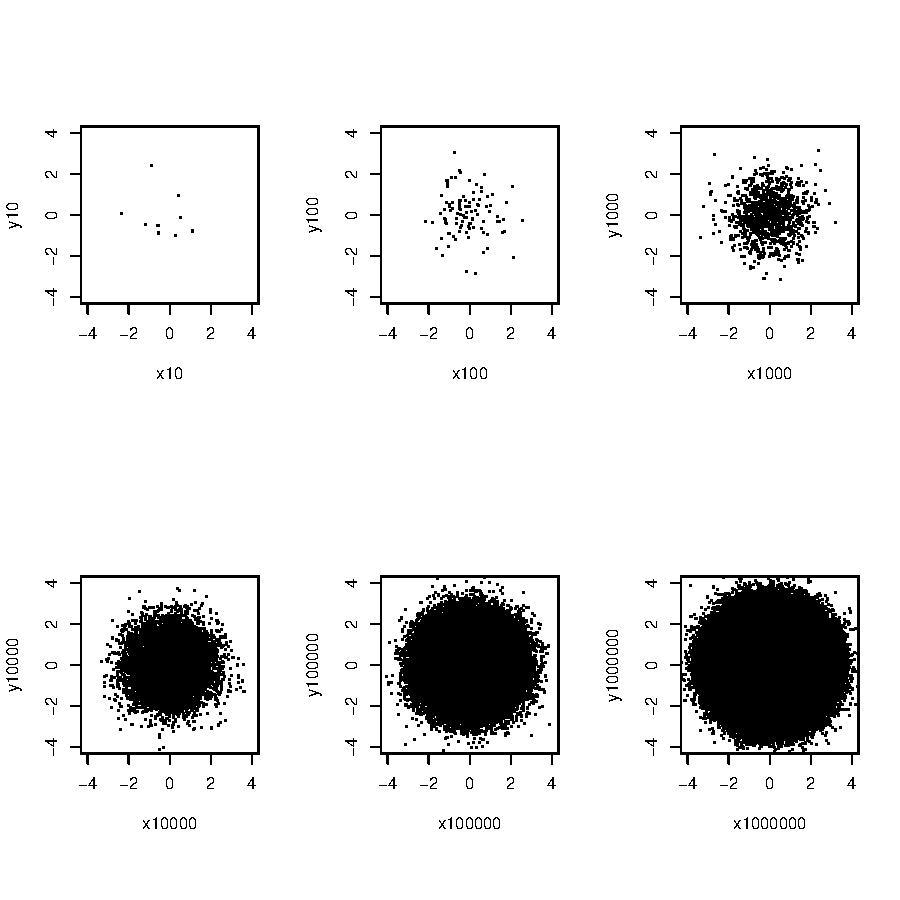
\includegraphics{lect_main-003}

See here for additional references: \\
\url{http://en.wikipedia.org/wiki/Anscombe's_quartet}
%\url{http://pbil.univ-lyon1.fr/library/base/html/anscombe.html}


\cite{Tu83}, p.~13, concludes: 
\begin{quotation}
``Graphics {\it reveal} data. Indeed graphics can be more precise and 
revealing than conventional statistical computations. Consider
Anscombe's quartet: all four of these data sets are described by 
exactly the same linear model (at least until the residuals are 
examined).''
\end{quotation}

The Anscombe data show up in numerous textbooks, as
early as in \cite{Tu74}, pp.~131--134, and as recent as
in \cite{MMC2012}, p.~120 (Exercise 2.73).
In fact, this data set should be shown in every undergraduate
class as well as in every regression class to demonstrate
what might happen when blindly performing any statistical
calculations without plotting the data first.


\else
{\bf Additional details will be provided after class.}
\fi


\newpage


\subsection{Further Reading}

In addition to \cite{Un2015}
cited so far in this chapter, many other sources exist that
make a strong case why to use graphics. 
Some of these additional sources are:

\begin{itemize}
\item \cite{Ans73}

\item \cite{Tuk77}

\end{itemize}



\begin{figure}[ht]
\centering{\includegraphics[width=4.0in]{Scans//AmstatNews_Jan2009_p25_Fig.jpg}}
\caption{\label{AmstatNews_Jan2009_p25_Fig}
Amstat News, January 2009, p.~25, Cartoon.
}
\end{figure}


\newpage


%\begin{sidewaysfigure}
%\begin{center}
%\includegraphics[height=0.5\textwidth]{Scans//AmstatNews_Jan2009_p25_Fig.jpg}
%\end{center}
%\hspace{1.5in}\parbox{6in}{\caption{\label{AmstatNews_Jan2009_p25_Fig}
%This is the rotated caption. This is the rotated caption. 
%This is the rotated caption. This is the rotated caption. 
%This is the rotated caption. This is the rotated caption.}}
%\end{sidewaysfigure}



% !Rnw root = lect_main.Rnw

\def\jsprivatechunwinone{1} % show additional details
%\def\jsprivatechunwinone{0} % do NOT show additional details



\section{Basic Graph Construction and Refinement}

{\bf (Based on \cite{Un2015}, Chapter 1: Setting the Scene}

The supporting materials for \cite{Un2015} can be obtained from
\url{http://www.gradaanwr.net/}.
In particular, the original R code for each chapter can be downloaded
as a zip file from
\url{http://www.gradaanwr.net/content/}.
We will work with modified versions of some of the provided code in class.


\subsection{Figure 1.1}


\begin{verbatim}
World Speed Skiing Competition, Verbier 21st April, 2011

Description
There were separate Speed Skiing competitions for men (79 participants) and 
women (12 participants).

Usage
data(SpeedSki)
\end{verbatim}


\begin{Schunk}
\begin{Sinput}
> ##Libraries
> library(ggplot2)
> library(gridExtra)
> library(ggthemes)
> library(dplyr)
> library(GGally)
> library(vcd)
> library(extracat)
> library(GDAdata)
> library(plotly)
> ##Settings
> palette("default")
> update_geom_defaults("bar", list(fill = "grey70", colour = "grey40"))
> scale_colour_discrete <- function(...) scale_colour_brewer(..., palette = "Set2")
> scale_fill_discrete <- function(...) scale_fill_colorblind()
> auTheme <- theme_grey()  + 
+   theme(panel.background = element_rect(colour = NA, fill = "grey90")) +
+   theme(plot.background = element_rect(colour = NA, fill = "grey90")) +
+   theme(legend.background = element_rect(fill = "grey90")) +
+   theme(plot.title = element_text(vjust = 2)) 
> theme_set(auTheme)
> ## ----speedski---- Fig 1.1
> data(SpeedSki, package = "GDAdata")
> # step-by-step
> 
> # basic first graphic
> ggplot(SpeedSki, aes(x = Speed)) +
+   geom_histogram()
> # adjust range of x-axis
> summary(SpeedSki$Speed)
\end{Sinput}
\begin{Soutput}
   Min. 1st Qu.  Median    Mean 3rd Qu.    Max. 
  160.2   171.8   183.1   184.1   192.3   211.7 
\end{Soutput}
\begin{Sinput}
> ggplot(SpeedSki, aes(x = Speed)) +
+   xlim(160, 220) +
+   geom_histogram()
> # adjust binwidth
> ggplot(SpeedSki, aes(x = Speed)) +
+   xlim(160, 220) +
+   geom_histogram(binwidth = 2.5)
> # add axis labels
> ggplot(SpeedSki, aes(x = Speed)) +
+   xlim(160, 220) + 
+   geom_histogram(binwidth = 2.5) +
+   xlab("Speed (km/hr)") + 
+   ylab("")
> # condition on gender in 2 related histograms (small multiples!)
> ggplot(SpeedSki, aes(x = Speed)) +
+   xlim(160, 220) + 
+   geom_histogram(binwidth = 2.5) +
+   xlab("Speed (km/hr)") + 
+   ylab("") +
+   facet_wrap(~ Sex, ncol = 1)
> # use color as a distinction for gender
> ggplot(SpeedSki, aes(x = Speed, fill = Sex)) +
+   xlim(160, 220) + 
+   geom_histogram(binwidth = 2.5) +
+   xlab("Speed (km/hr)") + 
+   ylab("") +
+   facet_wrap(~ Sex, ncol = 1)
> # omit legend = code from the book
> ggplot(SpeedSki, aes(x = Speed, fill = Sex)) +
+   xlim(160, 220) + 
+   geom_histogram(binwidth = 2.5) +
+   xlab("Speed (km/hr)") + 
+   ylab("") +
+   facet_wrap(~ Sex, ncol = 1) +
+   theme(legend.position = "none")
> # final result in book
> ggplot(SpeedSki, aes(x = Speed, fill = Sex)) + 
+   xlim(160, 220) +
+   geom_histogram(binwidth = 2.5, center = 1.25) + 
+   xlab("Speed (km/hr)") + 
+   ylab("") +
+   facet_wrap(~ Sex, ncol = 1) + 
+   theme(legend.position = "none")
> # further adjust y-axis range
> ggplot(SpeedSki, aes(x = Speed, fill = Sex)) + 
+   xlim(160, 220) +
+   ylim(0, 12) +
+   geom_histogram(binwidth = 2.5, center = 1.25) + 
+   xlab("Speed (km/hr)") + 
+   ylab("") +
+   facet_wrap(~ Sex, ncol = 1) + 
+   theme(legend.position = "none")
> # further adjust y-axis ticks & gridlines
> ggplot(SpeedSki, aes(x = Speed, fill = Sex)) + 
+   xlim(160, 220) +
+   ylim(0, 12) +
+   scale_y_continuous(breaks = seq(0, 12, 2)) +
+   geom_histogram(binwidth = 2.5, center = 1.25) + 
+   xlab("Speed (km/hr)") + 
+   ylab("") +
+   facet_wrap(~ Sex, ncol = 1) + 
+   theme(legend.position = "none")
> # interactive version
> ggplotly()
> # save as external jpg file
> jpeg("Speedski.jpg")
> ggplot(SpeedSki, aes(x = Speed, fill = Sex)) + 
+   xlim(160, 220) +
+   ylim(0, 12) +
+   scale_y_continuous(breaks = seq(0, 12, 2)) +
+   geom_histogram(binwidth = 2.5, center = 1.25) + 
+   xlab("Speed (km/hr)") + 
+   ylab("") +
+   facet_wrap(~ Sex, ncol = 1) + 
+   theme(legend.position = "none")
> dev.off()
\end{Sinput}
\begin{Soutput}
pdf 
  2 
\end{Soutput}
\begin{Sinput}
> # save as external pdf file
> pdf("Speedski.pdf")
> ggplot(SpeedSki, aes(x = Speed, fill = Sex)) + 
+   xlim(160, 220) +
+   ylim(0, 12) +
+   scale_y_continuous(breaks = seq(0, 12, 2)) +
+   geom_histogram(binwidth = 2.5, center = 1.25) + 
+   xlab("Speed (km/hr)") + 
+   ylab("") +
+   facet_wrap(~ Sex, ncol = 1) + 
+   theme(legend.position = "none")
> dev.off()
\end{Sinput}
\begin{Soutput}
pdf 
  2 
\end{Soutput}
\begin{Sinput}
> # Question: How to extract the intervals from a ggplot histogram object?
> # Answer based on: https://stackoverflow.com/questions/25378184/need-to-extract-data-from-the-ggplot-geom-histogram
> 
> # assign ggplot object to a variable
> g <- ggplot(SpeedSki, aes(x = Speed)) +
+   geom_histogram()
> class(g)
\end{Sinput}
\begin{Soutput}
[1] "gg"     "ggplot"
\end{Soutput}
\begin{Sinput}
> g
> # extract plot information
> pg <- ggplot_build(g)
> class(pg)
\end{Sinput}
\begin{Soutput}
[1] "ggplot_built"
\end{Soutput}
\begin{Sinput}
> names(pg)
\end{Sinput}
\begin{Soutput}
[1] "data"   "layout" "plot"  
\end{Soutput}
\begin{Sinput}
> # look at the data part
> head(pg$data[[1]])
\end{Sinput}
\begin{Soutput}
  y count        x     xmin     xmax  density    ncount  ndensity PANEL group
1 1     1 159.6724 158.7853 160.5595 0.006194 0.1111111 0.1111111     1    -1
2 1     1 161.4466 160.5595 162.3336 0.006194 0.1111111 0.1111111     1    -1
3 1     1 163.2207 162.3336 164.1078 0.006194 0.1111111 0.1111111     1    -1
4 4     4 164.9948 164.1078 165.8819 0.024776 0.4444444 0.4444444     1    -1
5 5     5 166.7690 165.8819 167.6560 0.030970 0.5555556 0.5555556     1    -1
6 6     6 168.5431 167.6560 169.4302 0.037164 0.6666667 0.6666667     1    -1
  ymin ymax   fill colour size linetype alpha
1    0    1 grey70 grey40  0.5        1    NA
2    0    1 grey70 grey40  0.5        1    NA
3    0    1 grey70 grey40  0.5        1    NA
4    0    4 grey70 grey40  0.5        1    NA
5    0    5 grey70 grey40  0.5        1    NA
6    0    6 grey70 grey40  0.5        1    NA
\end{Soutput}
\begin{Sinput}
> # compare with the modified intervals
> 
> g2 <- ggplot(SpeedSki, aes(x = Speed, fill = Sex)) + 
+   xlim(160, 220) +
+   geom_histogram(binwidth = 2.5, center = 1.25) + 
+   xlab("Speed (km/hr)") + 
+   ylab("") +
+   facet_wrap(~ Sex, ncol = 1) + 
+   theme(legend.position = "none")
> g2
> pg2 <- ggplot_build(g2)
> head(pg2$data[[1]])
\end{Sinput}
\begin{Soutput}
     fill y count      x  xmin  xmax    density    ncount  ndensity PANEL group
1 #000000 3     3 161.25 160.0 162.5 0.10000000 1.0000000 1.0000000     1     1
2 #000000 0     0 163.75 162.5 165.0 0.00000000 0.0000000 0.0000000     1     1
3 #000000 1     1 166.25 165.0 167.5 0.03333333 0.3333333 0.3333333     1     1
4 #000000 1     1 168.75 167.5 170.0 0.03333333 0.3333333 0.3333333     1     1
5 #000000 0     0 171.25 170.0 172.5 0.00000000 0.0000000 0.0000000     1     1
6 #000000 0     0 173.75 172.5 175.0 0.00000000 0.0000000 0.0000000     1     1
  ymin ymax colour size linetype alpha
1    0    3 grey40  0.5        1    NA
2    0    0 grey40  0.5        1    NA
3    0    1 grey40  0.5        1    NA
4    0    1 grey40  0.5        1    NA
5    0    0 grey40  0.5        1    NA
6    0    0 grey40  0.5        1    NA
\end{Soutput}
\begin{Sinput}
> ## BaseR
> 
> # basic first graphic
> hist(SpeedSki$Speed)
> # adjust range of x-axis & binwidth
> hist(SpeedSki$Speed,
+      breaks = seq(160, 220, by = 2.5))
> # add axis labels
> hist(SpeedSki$Speed,
+      breaks = seq(160, 220, by = 2.5),
+      xlab = "Speed (km/hr)",
+      ylab = "")
> # condition on gender in 2 related histograms (small multiples!)
> hist(SpeedSki$Speed[SpeedSki$Sex == "Female"],
+      breaks = seq(160, 220, by = 2.5),
+      xlab = "Speed (km/hr)",
+      ylab = "")
> hist(SpeedSki$Speed[SpeedSki$Sex == "Male"],
+      breaks = seq(160, 220, by = 2.5),
+      xlab = "Speed (km/hr)",
+      ylab = "")
> # combine into 1 figure
> op <- par(no.readonly = TRUE) # save original graphical parameters
> par(mfrow = c(2, 1))
> hist(SpeedSki$Speed[SpeedSki$Sex == "Female"],
+      breaks = seq(160, 220, by = 2.5),
+      xlab = "Speed (km/hr)",
+      ylab = "")
> hist(SpeedSki$Speed[SpeedSki$Sex == "Male"],
+      breaks = seq(160, 220, by = 2.5),
+      xlab = "Speed (km/hr)",
+      ylab = "")
> # add individual main titles
> par(mfrow = c(2, 1))
> hist(SpeedSki$Speed[SpeedSki$Sex == "Female"],
+      breaks = seq(160, 220, by = 2.5),
+      xlab = "Speed (km/hr)",
+      ylab = "",
+      main = "Female")
> hist(SpeedSki$Speed[SpeedSki$Sex == "Male"],
+      breaks = seq(160, 220, by = 2.5),
+      xlab = "Speed (km/hr)",
+      ylab = "",
+      main = "Male")
> # adjust y-axis to common scale (small multiples!)
> par(mfrow = c(2, 1))
> hist(SpeedSki$Speed[SpeedSki$Sex == "Female"],
+      breaks = seq(160, 220, by = 2.5),
+      ylim = c(0, 12),
+      xlab = "Speed (km/hr)",
+      ylab = "",
+      main = "Female")
> hist(SpeedSki$Speed[SpeedSki$Sex == "Male"],
+      breaks = seq(160, 220, by = 2.5),
+      ylim = c(0, 12),
+      xlab = "Speed (km/hr)",
+      ylab = "",
+      main = "Male")
> # reduce outer margins # c(bottom, left, top, right)
> par(mfrow = c(2, 1),
+     oma = c(0, 0, 0, 0))
> hist(SpeedSki$Speed[SpeedSki$Sex == "Female"],
+      breaks = seq(160, 220, by = 2.5),
+      ylim = c(0, 12),
+      xlab = "Speed (km/hr)",
+      ylab = "",
+      main = "Female")
> hist(SpeedSki$Speed[SpeedSki$Sex == "Male"],
+      breaks = seq(160, 220, by = 2.5),
+      ylim = c(0, 12),
+      xlab = "Speed (km/hr)",
+      ylab = "",
+      main = "Male")
> # reduce inner margins # c(bottom, left, top, right)
> par(mfrow = c(2, 1),
+     oma = c(0, 0, 0, 0),
+     mar = c(5, 3, 1, 0))
> hist(SpeedSki$Speed[SpeedSki$Sex == "Female"],
+      breaks = seq(160, 220, by = 2.5),
+      ylim = c(0, 12),
+      xlab = "Speed (km/hr)",
+      ylab = "",
+      main = "Female")
> hist(SpeedSki$Speed[SpeedSki$Sex == "Male"],
+      breaks = seq(160, 220, by = 2.5),
+      ylim = c(0, 12),
+      xlab = "Speed (km/hr)",
+      ylab = "",
+      main = "Male")
> par(op) # reset par for future graphics 
\end{Sinput}
\end{Schunk}


\subsection{Figure 1.2}


\begin{Schunk}
\begin{Sinput}
> ## ----speedski2---- Fig 1.2
> 
> # final result in book for Fig 1.1
> ggplot(SpeedSki, aes(x = Speed, fill = Sex)) + 
+   xlim(160, 220) +
+   geom_histogram(binwidth = 2.5, center = 1.25) + 
+   xlab("Speed (km/hr)") + 
+   ylab("") +
+   facet_wrap(~ Sex, ncol = 1) + 
+   theme(legend.position = "none")
> # different layout
> ggplot(SpeedSki, aes(x = Speed, fill = Sex)) + 
+   xlim(160, 220) +
+   geom_histogram(binwidth = 2.5, center = 1.25) + 
+   xlab("Speed (km/hr)") + 
+   ylab("") +
+   facet_grid(~ Sex) + 
+   theme(legend.position = "none")
> # condition on event
> ggplot(SpeedSki, aes(Speed, fill = Sex)) +
+   geom_histogram(binwidth = 2.5)  + 
+   xlab("Speed (km/hr)") +
+   ylab("") + 
+   facet_grid(Sex ~ Event) +
+   theme(legend.position = "none")
> # readjust range and center of bins
> ggplot(SpeedSki, aes(Speed, fill = Sex)) +
+   xlim(160, 220) +
+   geom_histogram(binwidth = 2.5, center = 1.25)  + 
+   xlab("Speed (km/hr)") +
+   ylab("") + 
+   facet_grid(Sex ~ Event) +
+   theme(legend.position = "none")
> # interactive version
> ggplotly()
> #try a few things yourself!
> names(SpeedSki)
\end{Sinput}
\begin{Soutput}
 [1] "Rank"       "Bib"        "FIS.Code"   "Name"       "Year"      
 [6] "Nation"     "Speed"      "Sex"        "Event"      "no.of.runs"
\end{Soutput}
\begin{Sinput}
> head(SpeedSki)
\end{Sinput}
\begin{Soutput}
  Rank Bib FIS.Code                 Name Year Nation  Speed  Sex     Event
1    1  61     7039       ORIGONE Simone 1979    ITA 211.67 Male Speed One
2    2  59     7078         ORIGONE Ivan 1987    ITA 209.70 Male Speed One
3    3  66   190130       MONTES Bastien 1985    FRA 209.69 Male Speed One
4    4  57     7178 SCHROTTSHAMMER Klaus 1979    AUT 209.67 Male Speed One
5    5  69   510089         MAY Philippe 1970    SUI 209.19 Male Speed One
6    6  75     7204          BILLY Louis 1993    FRA 208.33 Male Speed One
  no.of.runs
1          4
2          4
3          4
4          4
5          4
6          4
\end{Soutput}
\begin{Sinput}
> ggplot(SpeedSki, aes(Speed, fill = Sex)) +
+   xlim(160, 220) +
+   geom_histogram(binwidth = 2.5, center = 1.25)  + 
+   xlab("Speed (km/hr)") +
+   ylab("") + 
+   facet_grid(Sex ~ no.of.runs ~ Event) +
+   theme(legend.position = "none")
> ggplot(SpeedSki, aes(Speed, fill = Sex)) +
+   xlim(160, 220) +
+   geom_histogram(binwidth = 2.5, center = 1.25)  + 
+   xlab("Speed (km/hr)") +
+   ylab("") + 
+   facet_grid(Sex ~ Nation ~ Event) +
+   theme(legend.position = "none")
\end{Sinput}
\end{Schunk}


\subsection{Figure 1.3}


\begin{verbatim}
Edgar Anderson's Iris Data

Description
This famous (Fisher's or Anderson's) iris data set gives the measurements 
in centimeters of the variables sepal length and width and petal length and width, 
respectively, for 50 flowers from each of 3 species of iris. The species are 
Iris setosa, versicolor, and virginica.

Usage
iris
iris3
\end{verbatim}


\begin{Schunk}
\begin{Sinput}
> ## ----petal1---- Fig 1.3
> 
> # basic first graphic = code from book
> ggplot(iris, aes(Petal.Length)) + 
+   geom_histogram()
> # adjust binwidth & center
> ggplot(iris, aes(Petal.Length)) + 
+   geom_histogram(binwidth = 0.5, center = 0.25)
> # adjust xlim & ylim 
> ggplot(iris, aes(Petal.Length)) + 
+   xlim(0, 8) +
+   ylim(0, 40) +
+   geom_histogram(binwidth = 0.5, center = 0.25)
> # interesting: notice the following
> summary(iris$Petal.Length)
\end{Sinput}
\begin{Soutput}
   Min. 1st Qu.  Median    Mean 3rd Qu.    Max. 
  1.000   1.600   4.350   3.758   5.100   6.900 
\end{Soutput}
\begin{Sinput}
> # interactive version
> ggplotly()
> ## BaseR
> 
> # basic first graphic
> hist(iris$Petal.Length)
> # add axis label & title
> hist(iris$Petal.Length,
+      xlab = "Petal Length",
+      main = "Iris Data Set")
> # adjust y-axis range
> hist(iris$Petal.Length,
+      ylim = c(0, 40),
+      xlab = "Petal Length",
+      main = "Iris Data Set")
> # adjust starting interval for x-axis
> hist(iris$Petal.Length,
+      breaks = seq(0, 7, by = 0.5),
+      ylim = c(0, 40),
+      xlab = "Petal Length",
+      main = "Iris Data Set")
\end{Sinput}
\end{Schunk}


\subsection{Figure 1.4}


\begin{Schunk}
\begin{Sinput}
> ## ----scpetal---- Fig 1.4
> 
> # basic first graphic
> ggplot(iris, aes(Petal.Length, Petal.Width)) +
+   geom_point() 
> # add color to distinguish species
> ggplot(iris, aes(Petal.Length, Petal.Width, color = Species)) +
+   geom_point() 
> # place legend at bottom
> ggplot(iris, aes(Petal.Length, Petal.Width, color = Species)) +
+   geom_point() + 
+   theme(legend.position = "bottom")
> # choose a different color scheme for colorblind viewers = code from book
> ggplot(iris, aes(Petal.Length, Petal.Width, color = Species)) +
+   geom_point() + 
+   theme(legend.position = "bottom") +
+   scale_colour_colorblind()
> # interactive version
> ggplotly()
> # try a few things
> ggplot(iris, aes(Petal.Length, Petal.Width, shape = Species)) +
+   geom_point() + 
+   theme(legend.position = "bottom")
> ggplot(iris, aes(Petal.Length, Petal.Width, shape = Species, color = Species)) +
+   geom_point() + 
+   theme(legend.position = "bottom")
> ggplot(iris, aes(Petal.Length, Petal.Width, shape = Species, color = Species, size = Sepal.Width)) +
+   geom_point() + 
+   theme(legend.position = "bottom")
> ## BaseR
> 
> # basic plot
> plot(iris$Petal.Length, iris$Petal.Width)
> # add color to distinguish species
> plot(iris$Petal.Length, iris$Petal.Width,
+      col = iris$Species)
> # add axis labels & title
> plot(iris$Petal.Length, iris$Petal.Width,
+      col = iris$Species,
+      xlab = "Petal Length",
+      ylab = "Petal Width",
+      main = "Iris Data")
\end{Sinput}
\end{Schunk}


\subsection{Figure 1.5}


\begin{verbatim}
Student Admissions at UC Berkeley

Description
Aggregate data on applicants to graduate school at Berkeley for the six largest 
departments in 1973 classified by admission and sex.

Usage
UCBAdmissions
\end{verbatim}


\begin{Schunk}
\begin{Sinput}
> ## ----ucbaDeptx---- Fig 1.5
> 
> # basic first graphics
> ucba <- as.data.frame(UCBAdmissions)
> a <- ggplot(ucba, aes(Dept)) + 
+   geom_bar(aes(weight = Freq))
> b <- ggplot(ucba, aes(Gender)) + 
+   geom_bar(aes(weight = Freq))
> c <- ggplot(ucba, aes(Admit)) + 
+   geom_bar(aes(weight = Freq))
> a
> b
> c
> # arrange layout
> ucba <- as.data.frame(UCBAdmissions)
> a <- ggplot(ucba, aes(Dept)) + 
+   geom_bar(aes(weight = Freq))
> b <- ggplot(ucba, aes(Gender)) + 
+   geom_bar(aes(weight = Freq))
> c <- ggplot(ucba, aes(Admit)) + 
+   geom_bar(aes(weight = Freq))
> grid.arrange(a, b, c)
> # refine layout
> ucba <- as.data.frame(UCBAdmissions)
> a <- ggplot(ucba, aes(Dept)) + 
+   geom_bar(aes(weight = Freq))
> b <- ggplot(ucba, aes(Gender)) + 
+   geom_bar(aes(weight = Freq))
> c <- ggplot(ucba, aes(Admit)) + 
+   geom_bar(aes(weight = Freq))
> grid.arrange(a, b, c, nrow = 1)
> # adjust widths = code from book
> ucba <- as.data.frame(UCBAdmissions)
> a <- ggplot(ucba, aes(Dept)) + 
+   geom_bar(aes(weight = Freq))
> b <- ggplot(ucba, aes(Gender)) + 
+   geom_bar(aes(weight = Freq))
> c <- ggplot(ucba, aes(Admit)) + 
+   geom_bar(aes(weight = Freq))
> grid.arrange(a, b, c, nrow = 1, widths = c(7, 3, 3))
\end{Sinput}
\end{Schunk}


\subsection{Figure 1.6}


\begin{Schunk}
\begin{Sinput}
> ## ----berkeleyS---- Fig 1.6
> 
> # basic first graphic
> ucb <- data.frame(UCBAdmissions)
> doubledecker(xtabs(Freq ~ Dept + Gender + Admit, data = ucb))
> # modify colors
> ucb <- data.frame(UCBAdmissions)
> doubledecker(xtabs(Freq ~ Dept + Gender + Admit, data = ucb),
+              gp = gpar(fill = c("grey90", "steelblue")))
> # create new factor with differently sorted levels and swap top/bottom in bars
> ucb <- data.frame(UCBAdmissions)
> ucb <- within(ucb, Accept <- 
+                 factor(Admit, levels = c("Rejected", "Admitted")))
> doubledecker(xtabs(Freq ~ Dept + Gender + Accept, data = ucb),
+              gp = gpar(fill = c("grey90", "steelblue")))
\end{Sinput}
\end{Schunk}


\subsection{Figure 1.7}


\begin{verbatim}
Diabetes in Pima Indian Women

Description
A population of women who were at least 21 years old, of Pima Indian heritage 
and living near Phoenix, Arizona, was tested for diabetes according to 
World Health Organization criteria. The data were collected by the 
US National Institute of Diabetes and Digestive and Kidney Diseases. 
We used the 532 complete records after dropping the (mainly missing) data on 
serum insulin.

Usage
Pima.tr
Pima.tr2
Pima.te
\end{verbatim}


\begin{Schunk}
\begin{Sinput}
> ## ----pimaHist---- Fig 1.7
> 
> # basic first graphics
> data(Pima.tr2, package = "MASS")
> h1 <- ggplot(Pima.tr2, aes(glu)) + 
+   geom_histogram()
> h2 <- ggplot(Pima.tr2, aes(bp)) + 
+   geom_histogram()
> h3 <- ggplot(Pima.tr2, aes(skin)) + 
+   geom_histogram()
> h4 <- ggplot(Pima.tr2, aes(bmi)) + 
+   geom_histogram()
> h5 <- ggplot(Pima.tr2, aes(ped)) + 
+   geom_histogram()
> h6 <- ggplot(Pima.tr2, aes(age)) + 
+   geom_histogram()
> h1
> h2 
> h3
> h4
> h5
> h6
> # arrange layout
> data(Pima.tr2, package = "MASS")
> h1 <- ggplot(Pima.tr2, aes(glu)) + 
+   geom_histogram()
> h2 <- ggplot(Pima.tr2, aes(bp)) + 
+   geom_histogram()
> h3 <- ggplot(Pima.tr2, aes(skin)) + 
+   geom_histogram()
> h4 <- ggplot(Pima.tr2, aes(bmi)) + 
+   geom_histogram()
> h5 <- ggplot(Pima.tr2, aes(ped)) + 
+   geom_histogram()
> h6 <- ggplot(Pima.tr2, aes(age)) + 
+   geom_histogram()
> grid.arrange(h1, h2, h3, h4, h5, h6)
> # refine layout = code from book
> data(Pima.tr2, package = "MASS")
> h1 <- ggplot(Pima.tr2, aes(glu)) + 
+   geom_histogram()
> h2 <- ggplot(Pima.tr2, aes(bp)) + 
+   geom_histogram()
> h3 <- ggplot(Pima.tr2, aes(skin)) + 
+   geom_histogram()
> h4 <- ggplot(Pima.tr2, aes(bmi)) + 
+   geom_histogram()
> h5 <- ggplot(Pima.tr2, aes(ped)) + 
+   geom_histogram()
> h6 <- ggplot(Pima.tr2, aes(age)) + 
+   geom_histogram()
> grid.arrange(h1, h2, h3, h4, h5, h6, nrow = 2)
\end{Sinput}
\end{Schunk}


\subsection{Figure 1.8}


\begin{Schunk}
\begin{Sinput}
> ## ----pimaBoxs---- Fig 1.8
> 
> ## BaseR
> 
> # basic first graphic
> PimaV <- select(Pima.tr2, glu:age)
> boxplot(PimaV)
> # use standardized scale
> PimaV <- select(Pima.tr2, glu:age)
> boxplot(scale(PimaV))
> # change symbol and color for outliers
> PimaV <- select(Pima.tr2, glu:age)
> boxplot(scale(PimaV), pch = 16, outcol = "red")
> # reduce margins = code from book
> PimaV <- select(Pima.tr2, glu:age)
> par(mar = c(3.1, 4.1, 1.1, 2.1))
> boxplot(scale(PimaV), pch = 16, outcol = "red")
> ## ggplot2
> 
> # basic boxplot of glu (needs "var" as a dummy argument)
> PimaV <- select(Pima.tr2, glu:age)
> ggplot(PimaV, aes("var", glu)) +
+   geom_boxplot()
> # boxplot of glu with x-axis labels removed
> PimaV <- select(Pima.tr2, glu:age)
> ggplot(PimaV, aes("var", glu)) +
+   xlab("") +
+   scale_x_discrete(breaks = NULL) +
+   geom_boxplot()
> # all boxplots, arranged side-by-side
> PimaV <- select(Pima.tr2, glu:age)
> b1 <- ggplot(PimaV, aes("var", glu)) +
+   xlab("") +
+   scale_x_discrete(breaks = NULL) +
+   geom_boxplot()
> b2 <- ggplot(PimaV, aes("var", bp)) +
+   xlab("") +
+   scale_x_discrete(breaks = NULL) +
+   geom_boxplot()
> b3 <- ggplot(PimaV, aes("var", skin)) +
+   xlab("") +
+   scale_x_discrete(breaks = NULL) +
+   geom_boxplot()
> b4 <- ggplot(PimaV, aes("var", bmi)) +
+   xlab("") +
+   scale_x_discrete(breaks = NULL) +
+   geom_boxplot()
> b5 <- ggplot(PimaV, aes("var", ped)) +
+   xlab("") +
+   scale_x_discrete(breaks = NULL) +
+   geom_boxplot()
> b6 <- ggplot(PimaV, aes("var", age)) +
+   xlab("") +
+   scale_x_discrete(breaks = NULL) +
+   geom_boxplot()
> grid.arrange(b1, b2, b3, b4, b5, b6, ncol = 6)
> # use standardized scale
> PimaV <- select(Pima.tr2, glu:age)
> PimaV <- as.data.frame(scale(PimaV))
> b1 <- ggplot(PimaV, aes("var", glu)) +
+   xlab("") +
+   scale_x_discrete(breaks = NULL) +
+   geom_boxplot()
> b2 <- ggplot(PimaV, aes("var", bp)) +
+   xlab("") +
+   scale_x_discrete(breaks = NULL) +
+   geom_boxplot()
> b3 <- ggplot(PimaV, aes("var", skin)) +
+   xlab("") +
+   scale_x_discrete(breaks = NULL) +
+   geom_boxplot()
> b4 <- ggplot(PimaV, aes("var", bmi)) +
+   xlab("") +
+   scale_x_discrete(breaks = NULL) +
+   geom_boxplot()
> b5 <- ggplot(PimaV, aes("var", ped)) +
+   xlab("") +
+   scale_x_discrete(breaks = NULL) +
+   geom_boxplot()
> b6 <- ggplot(PimaV, aes("var", age)) +
+   xlab("") +
+   scale_x_discrete(breaks = NULL) +
+   geom_boxplot()
> grid.arrange(b1, b2, b3, b4, b5, b6, ncol = 6)
> # enforce y-range from -5 to 7.5
> PimaV <- select(Pima.tr2, glu:age)
> PimaV <- as.data.frame(scale(PimaV))
> b1 <- ggplot(PimaV, aes("var", glu)) +
+   xlab("") +
+   scale_x_discrete(breaks = NULL) +
+   ylim(-5, 7.5) +
+   geom_boxplot()
> b2 <- ggplot(PimaV, aes("var", bp)) +
+   xlab("") +
+   scale_x_discrete(breaks = NULL) +
+   ylim(-5, 7.5) +
+   geom_boxplot()
> b3 <- ggplot(PimaV, aes("var", skin)) +
+   xlab("") +
+   scale_x_discrete(breaks = NULL) +
+   ylim(-5, 7.5) +
+   geom_boxplot()
> b4 <- ggplot(PimaV, aes("var", bmi)) +
+   xlab("") +
+   scale_x_discrete(breaks = NULL) +
+   ylim(-5, 7.5) +
+   geom_boxplot()
> b5 <- ggplot(PimaV, aes("var", ped)) +
+   xlab("") +
+   scale_x_discrete(breaks = NULL) +
+   ylim(-5, 7.5) +
+   geom_boxplot()
> b6 <- ggplot(PimaV, aes("var", age)) +
+   xlab("") +
+   scale_x_discrete(breaks = NULL) +
+   ylim(-5, 7.5) +
+   geom_boxplot()
> grid.arrange(b1, b2, b3, b4, b5, b6, ncol = 6)
> ## ggplot2
> 
> # alternatively: reshape the data first
> PimaV <- select(Pima.tr2, glu:age)
> PimaV <- as.data.frame(scale(PimaV))
> head(PimaV)
\end{Sinput}
\begin{Soutput}
         glu         bp        skin        bmi        ped        age
1 -1.2576269 -0.3691372 -0.09873518 -0.2853660 -0.2432339 -0.7856735
2  2.3743082 -0.1982624  0.32925852 -1.0708354 -0.9255154  1.8917775
3 -1.5575115  0.8269863  1.01404844  0.5771102 -0.9492765  0.1643897
4  1.3746930  0.3143620  1.18524592  2.4406749 -0.5996496 -0.6129347
5 -0.5578963 -1.0526363 -0.35553140 -0.8706177 -1.0273485 -0.8720429
6 -0.8911014  0.3143620 -0.18433392  0.5463075 -0.1957118  1.6326693
\end{Soutput}
\begin{Sinput}
> PimaV <- reshape(PimaV, idvar = "number", 
+                  times = names(PimaV), 
+                  timevar = "variable", 
+                  varying = list(names(PimaV)), 
+                  direction = "long")
> head(PimaV)
\end{Sinput}
\begin{Soutput}
      variable        glu number
1.glu      glu -1.2576269      1
2.glu      glu  2.3743082      2
3.glu      glu -1.5575115      3
4.glu      glu  1.3746930      4
5.glu      glu -0.5578963      5
6.glu      glu -0.8911014      6
\end{Soutput}
\begin{Sinput}
> ggplot(PimaV, aes(variable, glu)) +
+   geom_boxplot()
> # rearrange order of factor levels
> PimaV <- select(Pima.tr2, glu:age)
> PimaV <- as.data.frame(scale(PimaV))
> PimaV <- reshape(PimaV, idvar = "number", 
+                  ids = row.names(PimaV),
+                  times = names(PimaV), 
+                  timevar = "variable", 
+                  varying = list(names(PimaV)), 
+                  v.names = "data",
+                  direction = "long")
> PimaV$variable <- as.factor(PimaV$variable)
> PimaV <- within(PimaV, newvariable <-
+                 factor(variable, levels = c("glu", "bp", "skin", "bmi", "ped", "age")))
> ggplot(PimaV, aes(newvariable, data)) +
+   geom_boxplot()
> # remove axis labels
> PimaV <- select(Pima.tr2, glu:age)
> PimaV <- as.data.frame(scale(PimaV))
> PimaV <- reshape(PimaV, idvar = "number", 
+                  ids = row.names(PimaV),
+                  times = names(PimaV), 
+                  timevar = "variable", 
+                  varying = list(names(PimaV)), 
+                  v.names = "data",
+                  direction = "long")
> PimaV$variable <- as.factor(PimaV$variable)
> PimaV <- within(PimaV, newvariable <-
+                 factor(variable, levels = c("glu", "bp", "skin", "bmi", "ped", "age")))
> ggplot(PimaV, aes(newvariable, data)) +
+   xlab("") +
+   ylab("") +
+   geom_boxplot()
> # change symbol and color for outliers
> PimaV <- select(Pima.tr2, glu:age)
> PimaV <- as.data.frame(scale(PimaV))
> PimaV <- reshape(PimaV, idvar = "number", 
+                  ids = row.names(PimaV),
+                  times = names(PimaV), 
+                  timevar = "variable", 
+                  varying = list(names(PimaV)), 
+                  v.names = "data",
+                  direction = "long")
> PimaV$variable <- as.factor(PimaV$variable)
> PimaV <- within(PimaV, newvariable <-
+                 factor(variable, levels = c("glu", "bp", "skin", "bmi", "ped", "age")))
> ggplot(PimaV, aes(newvariable, data)) +
+   xlab("") +
+   ylab("") +
+   geom_boxplot(outlier.shape = 16, outlier.color = "red")
> # interactive version
> ggplotly()
\end{Sinput}
\end{Schunk}


\subsection{Figure 1.9}


\begin{Schunk}
\begin{Sinput}
> ## ----pimaSpl---- Fig 1.9
> 
> # basic graphic
> PimaV <- select(Pima.tr2, glu:age)
> ggpairs(PimaV)
> # no visible changes, so these are the defaults
> PimaV <- select(Pima.tr2, glu:age)
> ggpairs(PimaV, diag = list(continuous = "density"),
+         axisLabels = "show")
> # interactive version
> ggplotly()
> ## BaseR
> 
> # basic scatterplot matrix
> pairs(PimaV)
\end{Sinput}
\end{Schunk}


\subsection{Additional Par and Layout Options for baseR}


\begin{Schunk}
\begin{Sinput}
> # Assume we want to plot 6 different plots at the same time
> 
> myPlots <- function(n = 6) {
+   set.seed(7777)
+   sapply(1:n, function(x) hist(rnorm(100, sd = x),
+                                xlab = "x Values",
+                                xlim = c(-20, 20),
+                                main = paste("Histogram", x)))
+ }
> dev.off()
\end{Sinput}
\begin{Soutput}
null device 
          1 
\end{Soutput}
\begin{Sinput}
> myPlots()
\end{Sinput}
\begin{Soutput}
         [,1]                 [,2]                 [,3]                
breaks   Numeric,13           Numeric,7            Numeric,8           
counts   Integer,12           Integer,6            Integer,7           
density  Numeric,12           Numeric,6            Numeric,7           
mids     Numeric,12           Numeric,6            Numeric,7           
xname    "rnorm(100, sd = x)" "rnorm(100, sd = x)" "rnorm(100, sd = x)"
equidist TRUE                 TRUE                 TRUE                
         [,4]                 [,5]                 [,6]                
breaks   Numeric,12           Numeric,8            Numeric,8           
counts   Integer,11           Integer,7            Integer,7           
density  Numeric,11           Numeric,7            Numeric,7           
mids     Numeric,11           Numeric,7            Numeric,7           
xname    "rnorm(100, sd = x)" "rnorm(100, sd = x)" "rnorm(100, sd = x)"
equidist TRUE                 TRUE                 TRUE                
\end{Soutput}
\begin{Sinput}
> # change layout with par() function
> 
> dev.off()
\end{Sinput}
\begin{Soutput}
null device 
          1 
\end{Soutput}
\begin{Sinput}
> par(mfrow = c(3, 2))
> myPlots()
\end{Sinput}
\begin{Soutput}
         [,1]                 [,2]                 [,3]                
breaks   Numeric,13           Numeric,7            Numeric,8           
counts   Integer,12           Integer,6            Integer,7           
density  Numeric,12           Numeric,6            Numeric,7           
mids     Numeric,12           Numeric,6            Numeric,7           
xname    "rnorm(100, sd = x)" "rnorm(100, sd = x)" "rnorm(100, sd = x)"
equidist TRUE                 TRUE                 TRUE                
         [,4]                 [,5]                 [,6]                
breaks   Numeric,12           Numeric,8            Numeric,8           
counts   Integer,11           Integer,7            Integer,7           
density  Numeric,11           Numeric,7            Numeric,7           
mids     Numeric,11           Numeric,7            Numeric,7           
xname    "rnorm(100, sd = x)" "rnorm(100, sd = x)" "rnorm(100, sd = x)"
equidist TRUE                 TRUE                 TRUE                
\end{Soutput}
\begin{Sinput}
> dev.off()
\end{Sinput}
\begin{Soutput}
null device 
          1 
\end{Soutput}
\begin{Sinput}
> par(mfrow = c(2, 3))
> myPlots()
\end{Sinput}
\begin{Soutput}
         [,1]                 [,2]                 [,3]                
breaks   Numeric,13           Numeric,7            Numeric,8           
counts   Integer,12           Integer,6            Integer,7           
density  Numeric,12           Numeric,6            Numeric,7           
mids     Numeric,12           Numeric,6            Numeric,7           
xname    "rnorm(100, sd = x)" "rnorm(100, sd = x)" "rnorm(100, sd = x)"
equidist TRUE                 TRUE                 TRUE                
         [,4]                 [,5]                 [,6]                
breaks   Numeric,12           Numeric,8            Numeric,8           
counts   Integer,11           Integer,7            Integer,7           
density  Numeric,11           Numeric,7            Numeric,7           
mids     Numeric,11           Numeric,7            Numeric,7           
xname    "rnorm(100, sd = x)" "rnorm(100, sd = x)" "rnorm(100, sd = x)"
equidist TRUE                 TRUE                 TRUE                
\end{Soutput}
\begin{Sinput}
> # adjust spacing around each plot
> 
> dev.off()
\end{Sinput}
\begin{Soutput}
null device 
          1 
\end{Soutput}
\begin{Sinput}
> par(mfrow = c(2, 3), mar = c(0, 0, 0, 0))
> myPlots()
\end{Sinput}
\begin{Soutput}
         [,1]                 [,2]                 [,3]                
breaks   Numeric,13           Numeric,7            Numeric,8           
counts   Integer,12           Integer,6            Integer,7           
density  Numeric,12           Numeric,6            Numeric,7           
mids     Numeric,12           Numeric,6            Numeric,7           
xname    "rnorm(100, sd = x)" "rnorm(100, sd = x)" "rnorm(100, sd = x)"
equidist TRUE                 TRUE                 TRUE                
         [,4]                 [,5]                 [,6]                
breaks   Numeric,12           Numeric,8            Numeric,8           
counts   Integer,11           Integer,7            Integer,7           
density  Numeric,11           Numeric,7            Numeric,7           
mids     Numeric,11           Numeric,7            Numeric,7           
xname    "rnorm(100, sd = x)" "rnorm(100, sd = x)" "rnorm(100, sd = x)"
equidist TRUE                 TRUE                 TRUE                
\end{Soutput}
\begin{Sinput}
> dev.off()
\end{Sinput}
\begin{Soutput}
null device 
          1 
\end{Soutput}
\begin{Sinput}
> par(mfrow = c(2, 3), mar = c(2, 1, 0, 0))
> myPlots()
\end{Sinput}
\begin{Soutput}
         [,1]                 [,2]                 [,3]                
breaks   Numeric,13           Numeric,7            Numeric,8           
counts   Integer,12           Integer,6            Integer,7           
density  Numeric,12           Numeric,6            Numeric,7           
mids     Numeric,12           Numeric,6            Numeric,7           
xname    "rnorm(100, sd = x)" "rnorm(100, sd = x)" "rnorm(100, sd = x)"
equidist TRUE                 TRUE                 TRUE                
         [,4]                 [,5]                 [,6]                
breaks   Numeric,12           Numeric,8            Numeric,8           
counts   Integer,11           Integer,7            Integer,7           
density  Numeric,11           Numeric,7            Numeric,7           
mids     Numeric,11           Numeric,7            Numeric,7           
xname    "rnorm(100, sd = x)" "rnorm(100, sd = x)" "rnorm(100, sd = x)"
equidist TRUE                 TRUE                 TRUE                
\end{Soutput}
\begin{Sinput}
> dev.off()
\end{Sinput}
\begin{Soutput}
null device 
          1 
\end{Soutput}
\begin{Sinput}
> par(mfrow = c(2, 3), mar = c(3, 2, 2, 0))
> myPlots()
\end{Sinput}
\begin{Soutput}
         [,1]                 [,2]                 [,3]                
breaks   Numeric,13           Numeric,7            Numeric,8           
counts   Integer,12           Integer,6            Integer,7           
density  Numeric,12           Numeric,6            Numeric,7           
mids     Numeric,12           Numeric,6            Numeric,7           
xname    "rnorm(100, sd = x)" "rnorm(100, sd = x)" "rnorm(100, sd = x)"
equidist TRUE                 TRUE                 TRUE                
         [,4]                 [,5]                 [,6]                
breaks   Numeric,12           Numeric,8            Numeric,8           
counts   Integer,11           Integer,7            Integer,7           
density  Numeric,11           Numeric,7            Numeric,7           
mids     Numeric,11           Numeric,7            Numeric,7           
xname    "rnorm(100, sd = x)" "rnorm(100, sd = x)" "rnorm(100, sd = x)"
equidist TRUE                 TRUE                 TRUE                
\end{Soutput}
\begin{Sinput}
> dev.off()
\end{Sinput}
\begin{Soutput}
null device 
          1 
\end{Soutput}
\begin{Sinput}
> par(mfrow = c(2, 3), mar = c(4, 4, 2, 0))
> myPlots()
\end{Sinput}
\begin{Soutput}
         [,1]                 [,2]                 [,3]                
breaks   Numeric,13           Numeric,7            Numeric,8           
counts   Integer,12           Integer,6            Integer,7           
density  Numeric,12           Numeric,6            Numeric,7           
mids     Numeric,12           Numeric,6            Numeric,7           
xname    "rnorm(100, sd = x)" "rnorm(100, sd = x)" "rnorm(100, sd = x)"
equidist TRUE                 TRUE                 TRUE                
         [,4]                 [,5]                 [,6]                
breaks   Numeric,12           Numeric,8            Numeric,8           
counts   Integer,11           Integer,7            Integer,7           
density  Numeric,11           Numeric,7            Numeric,7           
mids     Numeric,11           Numeric,7            Numeric,7           
xname    "rnorm(100, sd = x)" "rnorm(100, sd = x)" "rnorm(100, sd = x)"
equidist TRUE                 TRUE                 TRUE                
\end{Soutput}
\begin{Sinput}
> mtext("Histograms with 6 different SDs", 
+       outer = TRUE,
+       side = 3)
> # allow space for a title above the 6 plots
> 
> dev.off()
\end{Sinput}
\begin{Soutput}
null device 
          1 
\end{Soutput}
\begin{Sinput}
> par(mfrow = c(2, 3), mar = c(4, 4, 2, 0), oma = c(0, 0, 2, 0))
> myPlots()
\end{Sinput}
\begin{Soutput}
         [,1]                 [,2]                 [,3]                
breaks   Numeric,13           Numeric,7            Numeric,8           
counts   Integer,12           Integer,6            Integer,7           
density  Numeric,12           Numeric,6            Numeric,7           
mids     Numeric,12           Numeric,6            Numeric,7           
xname    "rnorm(100, sd = x)" "rnorm(100, sd = x)" "rnorm(100, sd = x)"
equidist TRUE                 TRUE                 TRUE                
         [,4]                 [,5]                 [,6]                
breaks   Numeric,12           Numeric,8            Numeric,8           
counts   Integer,11           Integer,7            Integer,7           
density  Numeric,11           Numeric,7            Numeric,7           
mids     Numeric,11           Numeric,7            Numeric,7           
xname    "rnorm(100, sd = x)" "rnorm(100, sd = x)" "rnorm(100, sd = x)"
equidist TRUE                 TRUE                 TRUE                
\end{Soutput}
\begin{Sinput}
> mtext("Histograms with 6 different SDs", 
+       outer = TRUE,
+       side = 3)
> dev.off()
\end{Sinput}
\begin{Soutput}
null device 
          1 
\end{Soutput}
\begin{Sinput}
> par(mfrow = c(2, 3), mar = c(4, 4, 2, 0), oma = c(0, 0, 2, 0))
> myPlots()
\end{Sinput}
\begin{Soutput}
         [,1]                 [,2]                 [,3]                
breaks   Numeric,13           Numeric,7            Numeric,8           
counts   Integer,12           Integer,6            Integer,7           
density  Numeric,12           Numeric,6            Numeric,7           
mids     Numeric,12           Numeric,6            Numeric,7           
xname    "rnorm(100, sd = x)" "rnorm(100, sd = x)" "rnorm(100, sd = x)"
equidist TRUE                 TRUE                 TRUE                
         [,4]                 [,5]                 [,6]                
breaks   Numeric,12           Numeric,8            Numeric,8           
counts   Integer,11           Integer,7            Integer,7           
density  Numeric,11           Numeric,7            Numeric,7           
mids     Numeric,11           Numeric,7            Numeric,7           
xname    "rnorm(100, sd = x)" "rnorm(100, sd = x)" "rnorm(100, sd = x)"
equidist TRUE                 TRUE                 TRUE                
\end{Soutput}
\begin{Sinput}
> mtext("Histograms with 6 different SDs", 
+       outer = TRUE,
+       side = 3,
+       cex = 1.5)
> dev.off()
\end{Sinput}
\begin{Soutput}
null device 
          1 
\end{Soutput}
\begin{Sinput}
> par(mfrow = c(2, 3), mar = c(4, 4, 2, 0), oma = c(0, 0, 3, 0))
> myPlots()
\end{Sinput}
\begin{Soutput}
         [,1]                 [,2]                 [,3]                
breaks   Numeric,13           Numeric,7            Numeric,8           
counts   Integer,12           Integer,6            Integer,7           
density  Numeric,12           Numeric,6            Numeric,7           
mids     Numeric,12           Numeric,6            Numeric,7           
xname    "rnorm(100, sd = x)" "rnorm(100, sd = x)" "rnorm(100, sd = x)"
equidist TRUE                 TRUE                 TRUE                
         [,4]                 [,5]                 [,6]                
breaks   Numeric,12           Numeric,8            Numeric,8           
counts   Integer,11           Integer,7            Integer,7           
density  Numeric,11           Numeric,7            Numeric,7           
mids     Numeric,11           Numeric,7            Numeric,7           
xname    "rnorm(100, sd = x)" "rnorm(100, sd = x)" "rnorm(100, sd = x)"
equidist TRUE                 TRUE                 TRUE                
\end{Soutput}
\begin{Sinput}
> mtext("Histograms with 6 different SDs", 
+       outer = TRUE,
+       side = 3,
+       line = 1,
+       cex = 1.5)
> # general layouts with layout() function
> 
> dev.off()
\end{Sinput}
\begin{Soutput}
null device 
          1 
\end{Soutput}
\begin{Sinput}
> graphics::layout(matrix(c(1, 1, 1, 2, 2, 3, 
+                           4, 5, 5, 6, 6, 6), 
+                         2, 6, byrow = TRUE)) 
> layout.show(6)
> myPlots()
\end{Sinput}
\begin{Soutput}
         [,1]                 [,2]                 [,3]                
breaks   Numeric,13           Numeric,7            Numeric,8           
counts   Integer,12           Integer,6            Integer,7           
density  Numeric,12           Numeric,6            Numeric,7           
mids     Numeric,12           Numeric,6            Numeric,7           
xname    "rnorm(100, sd = x)" "rnorm(100, sd = x)" "rnorm(100, sd = x)"
equidist TRUE                 TRUE                 TRUE                
         [,4]                 [,5]                 [,6]                
breaks   Numeric,12           Numeric,8            Numeric,8           
counts   Integer,11           Integer,7            Integer,7           
density  Numeric,11           Numeric,7            Numeric,7           
mids     Numeric,11           Numeric,7            Numeric,7           
xname    "rnorm(100, sd = x)" "rnorm(100, sd = x)" "rnorm(100, sd = x)"
equidist TRUE                 TRUE                 TRUE                
\end{Soutput}
\begin{Sinput}
> ### a rather complicated layout for 22 plots
> 
> dev.off()
\end{Sinput}
\begin{Soutput}
null device 
          1 
\end{Soutput}
\begin{Sinput}
> n3 <- rep(0, 3)
> n4 <- rep(0, 4)
> graphics::layout(matrix(c(n4, rep(1, 5), n3, rep(2, 5), n3, rep(3, 5), n3, rep(4, 5), n4,
+                           rep(5, 5), n3, rep(6, 5), n3, rep(7, 5), n3, rep(8, 5), n3, rep(9, 5),
+                           n4, rep(10, 5), n3, rep(11, 5), n3, rep(12, 5), n3, rep(13, 5), n4,
+                           rep(14, 5), n3, rep(15, 5), n3, rep(16, 5), n3, rep(17, 5), n3, rep(18, 5),
+                           n4, rep(19, 5), n3, rep(20, 5), n3, rep(21, 5), n3, rep(22, 5), n4),
+                         nrow = 5, byrow = TRUE))
> layout.show(22)
> par(mar = c(0, 0, 0, 0)) # should be adjusted to something more meaningful
> myPlots()
\end{Sinput}
\begin{Soutput}
         [,1]                 [,2]                 [,3]                
breaks   Numeric,13           Numeric,7            Numeric,8           
counts   Integer,12           Integer,6            Integer,7           
density  Numeric,12           Numeric,6            Numeric,7           
mids     Numeric,12           Numeric,6            Numeric,7           
xname    "rnorm(100, sd = x)" "rnorm(100, sd = x)" "rnorm(100, sd = x)"
equidist TRUE                 TRUE                 TRUE                
         [,4]                 [,5]                 [,6]                
breaks   Numeric,12           Numeric,8            Numeric,8           
counts   Integer,11           Integer,7            Integer,7           
density  Numeric,11           Numeric,7            Numeric,7           
mids     Numeric,11           Numeric,7            Numeric,7           
xname    "rnorm(100, sd = x)" "rnorm(100, sd = x)" "rnorm(100, sd = x)"
equidist TRUE                 TRUE                 TRUE                
\end{Soutput}
\begin{Sinput}
> myPlots()
\end{Sinput}
\begin{Soutput}
         [,1]                 [,2]                 [,3]                
breaks   Numeric,13           Numeric,7            Numeric,8           
counts   Integer,12           Integer,6            Integer,7           
density  Numeric,12           Numeric,6            Numeric,7           
mids     Numeric,12           Numeric,6            Numeric,7           
xname    "rnorm(100, sd = x)" "rnorm(100, sd = x)" "rnorm(100, sd = x)"
equidist TRUE                 TRUE                 TRUE                
         [,4]                 [,5]                 [,6]                
breaks   Numeric,12           Numeric,8            Numeric,8           
counts   Integer,11           Integer,7            Integer,7           
density  Numeric,11           Numeric,7            Numeric,7           
mids     Numeric,11           Numeric,7            Numeric,7           
xname    "rnorm(100, sd = x)" "rnorm(100, sd = x)" "rnorm(100, sd = x)"
equidist TRUE                 TRUE                 TRUE                
\end{Soutput}
\begin{Sinput}
> myPlots()
\end{Sinput}
\begin{Soutput}
         [,1]                 [,2]                 [,3]                
breaks   Numeric,13           Numeric,7            Numeric,8           
counts   Integer,12           Integer,6            Integer,7           
density  Numeric,12           Numeric,6            Numeric,7           
mids     Numeric,12           Numeric,6            Numeric,7           
xname    "rnorm(100, sd = x)" "rnorm(100, sd = x)" "rnorm(100, sd = x)"
equidist TRUE                 TRUE                 TRUE                
         [,4]                 [,5]                 [,6]                
breaks   Numeric,12           Numeric,8            Numeric,8           
counts   Integer,11           Integer,7            Integer,7           
density  Numeric,11           Numeric,7            Numeric,7           
mids     Numeric,11           Numeric,7            Numeric,7           
xname    "rnorm(100, sd = x)" "rnorm(100, sd = x)" "rnorm(100, sd = x)"
equidist TRUE                 TRUE                 TRUE                
\end{Soutput}
\begin{Sinput}
> myPlots(4)
\end{Sinput}
\begin{Soutput}
         [,1]                 [,2]                 [,3]                
breaks   Numeric,13           Numeric,7            Numeric,8           
counts   Integer,12           Integer,6            Integer,7           
density  Numeric,12           Numeric,6            Numeric,7           
mids     Numeric,12           Numeric,6            Numeric,7           
xname    "rnorm(100, sd = x)" "rnorm(100, sd = x)" "rnorm(100, sd = x)"
equidist TRUE                 TRUE                 TRUE                
         [,4]                
breaks   Numeric,12          
counts   Integer,11          
density  Numeric,11          
mids     Numeric,11          
xname    "rnorm(100, sd = x)"
equidist TRUE                
\end{Soutput}
\begin{Sinput}
> dev.off()
\end{Sinput}
\begin{Soutput}
null device 
          1 
\end{Soutput}
\end{Schunk}


\subsection{Exercise 1.1}


Iris: How would you describe this histogram of sepal width?

\begin{Schunk}
\begin{Sinput}
> ## ----irisEx---- Ex. 1
> ggplot(iris, aes(Sepal.Width)) +
+   geom_histogram(binwidth = 0.1)
> summary(iris$Sepal.Width)
\end{Sinput}
\begin{Soutput}
   Min. 1st Qu.  Median    Mean 3rd Qu.    Max. 
  2.000   2.800   3.000   3.057   3.300   4.400 
\end{Soutput}
\end{Schunk}


\subsection{Exercise 1.2}

Pima Indians: Summarize what this barchart shows:

\begin{Schunk}
\begin{Sinput}
> ## ----PimaEx---- Ex. 2
> ggplot(Pima.tr2, aes(type)) + 
+   geom_bar()
\end{Sinput}
\end{Schunk}


\subsection{Exercise 1.3}

Pima Indians: Why is the upper left of this plot of numbers of pregnancies against
age empty?

\begin{Schunk}
\begin{Sinput}
> ## ----Pima2Ex---- Ex. 3
> ggplot(Pima.tr2, aes(age, npreg)) + 
+   geom_point()
\end{Sinput}
\end{Schunk}


\subsection{Exercise 1.4}

Estimating the speed of light: There are 100 estimates of the speed of light made by
Michelson in 1879, composed of 5 groups of 20 experiments each (dataset michelson in the
MASS package).
\begin{enumerate}
\item What plot would you draw for showing the distribution of all the values together?
What conclusions would you draw?
\item What plots might be useful for comparing the estimates from the 5 different experiments?
Do the results from the 5 experiments look similar?
\end{enumerate}


\begin{verbatim}
Michelson's Speed of Light Data

Description
Measurements of the speed of light in air, made between 5th June and 2nd July, 1879. 
The data consists of five experiments, each consisting of 20 consecutive runs. 
The response is the speed of light in km/s, less 299000. The currently accepted 
value, on this scale of measurement, is 734.5.

Usage
michelson
\end{verbatim}

\begin{Schunk}
\begin{Sinput}
> data(michelson, package = "MASS")
> class(michelson)
\end{Sinput}
\begin{Soutput}
[1] "data.frame"
\end{Soutput}
\begin{Sinput}
> head(michelson)
\end{Sinput}
\begin{Soutput}
  Speed Run Expt
1   850   1    1
2   740   2    1
3   900   3    1
4  1070   4    1
5   930   5    1
6   850   6    1
\end{Soutput}
\begin{Sinput}
> summary(michelson)
\end{Sinput}
\begin{Soutput}
     Speed             Run     Expt  
 Min.   : 620.0   1      : 5   1:20  
 1st Qu.: 807.5   2      : 5   2:20  
 Median : 850.0   3      : 5   3:20  
 Mean   : 852.4   4      : 5   4:20  
 3rd Qu.: 892.5   5      : 5   5:20  
 Max.   :1070.0   6      : 5         
                  (Other):70         
\end{Soutput}
\begin{Sinput}
> ggplot(michelson, aes(Speed)) + 
+   geom_histogram()
> ggplot(michelson, aes(Speed)) + 
+   geom_histogram(binwidth = 25)
> ggplot(michelson, aes(Speed)) + 
+   geom_histogram(binwidth = 50)
> ggplot(michelson, aes(Speed)) + 
+   geom_histogram(binwidth = 50) +
+   facet_wrap(~ Expt, ncol = 3)
> ggplot(michelson, aes(Expt, Speed)) +
+   geom_boxplot()
> summary(michelson)
\end{Sinput}
\begin{Soutput}
     Speed             Run     Expt  
 Min.   : 620.0   1      : 5   1:20  
 1st Qu.: 807.5   2      : 5   2:20  
 Median : 850.0   3      : 5   3:20  
 Mean   : 852.4   4      : 5   4:20  
 3rd Qu.: 892.5   5      : 5   5:20  
 Max.   :1070.0   6      : 5         
                  (Other):70         
\end{Soutput}
\begin{Sinput}
> summary(michelson[michelson$Expt != "1", ])
\end{Sinput}
\begin{Soutput}
     Speed            Run     Expt  
 Min.   :620.0   1      : 4   1: 0  
 1st Qu.:800.0   2      : 4   2:20  
 Median :840.0   3      : 4   3:20  
 Mean   :838.2   4      : 4   4:20  
 3rd Qu.:880.0   5      : 4   5:20  
 Max.   :970.0   6      : 4         
                 (Other):56         
\end{Soutput}
\begin{Sinput}
> 
\end{Sinput}
\end{Schunk}


\newpage


~\\[2cm]


\begin{figure}[ht]
\centering{\includegraphics[height=4in]{Scans//Cartoonstock_ArtistRetreat.jpg}}
\caption{\label{Cartoonstock_ArtistRetreat}
\url{http://www.cartoonstock.com/blowup_stock.asp?imageref=hsc3714&artist=Schwadron,+Harley&topic=statistics+},
Cartoon.
}
\end{figure}


\newpage

%\SweaveInput{lect_chapter11.Rnw}
%\SweaveInput{lect_chapter4.Rnw}
%\SweaveInput{lect_chapter5.Rnw}
%\SweaveInput{lect_chapter6.Rnw}
%\SweaveInput{lect_chapter1.Rnw}
%
%\SweaveInput{lect_chapter2.Rnw}
%\SweaveInput{lect_chapter3.Rnw}
%\SweaveInput{lect_chapter9.Rnw}
%\SweaveInput{lect_chapter7.Rnw}
%\SweaveInput{lect_chapter8.Rnw}
%\SweaveInput{lect_chapter10.Rnw}


\setcounter{page}{1}
\addcontentsline{toc}{section}{References}

\bibliography{references}


\vspace*{1cm}

\centering{\bf \LARGE --- THE END ---}~\\[1cm]

\begin{figure}[ht]
\centering{\includegraphics[height=3in]{Scans//Cartoonstock_FallingArrow.jpg}}
\caption{\label{Cartoonstock_FallingArrow}
\url{http://www.cartoonstock.com/blowup_stock.asp?imageref=vsh0184&artist=Shirvanian,+Vahan&topic=statistics+}, 
Cartoon.
}
\end{figure}


\end{document}

